\graphicspath{{chapters/images/03/}}

\chapter{NGS principles (second gen. sequencing) - From Sanger to third gen sequencing}

\begin{figure}[h]
\caption{}
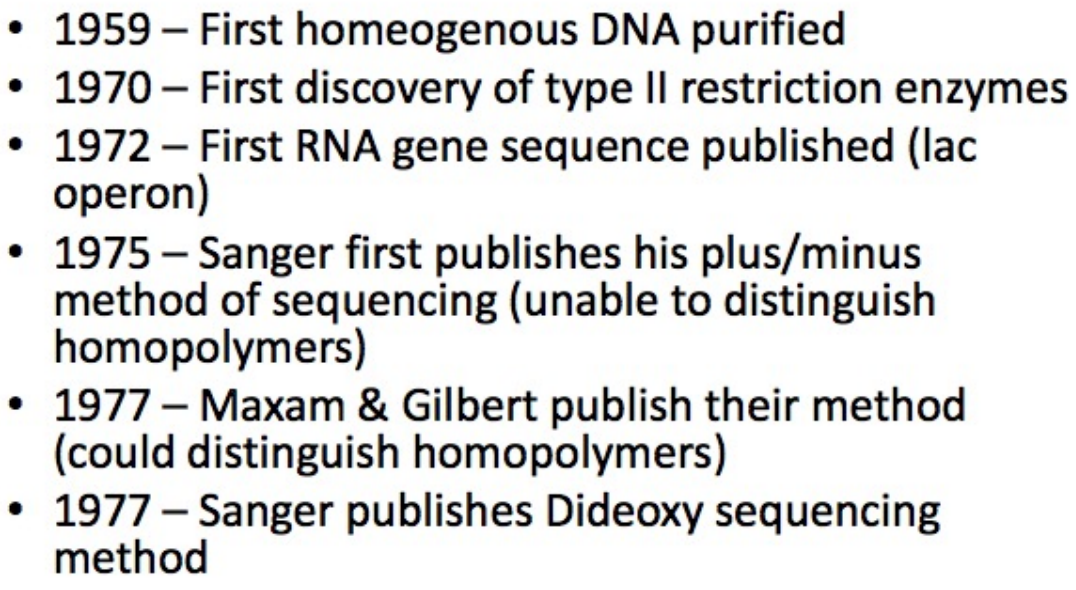
\includegraphics[width=0.6\textwidth]{history-seq}
\label{discoveries-sequencing}
\end{figure}

NGS stands for \textbf{\textit{Next Generation Sequencing}}, and it represents the method of sequencing most used nowadays. Before that, a series of other discoveries were done, elencated in the figure \ref{discoveries-sequencing}.

\section{History of Sequencing}
\subsection{Progresses of sequencing}
As the time passes, the cost of sequencing the DNA is diminishing. The rate of decrease actually is higher than the one predicted by the \textbf{Moore's Law}, \textit{"Democratization of sequencing"} is seen nowadays, because of the costs lowering. After the Human genome project, several other animals and plants' genomes were sequenced.

\begin{figure}[h]
\caption{}
\centering
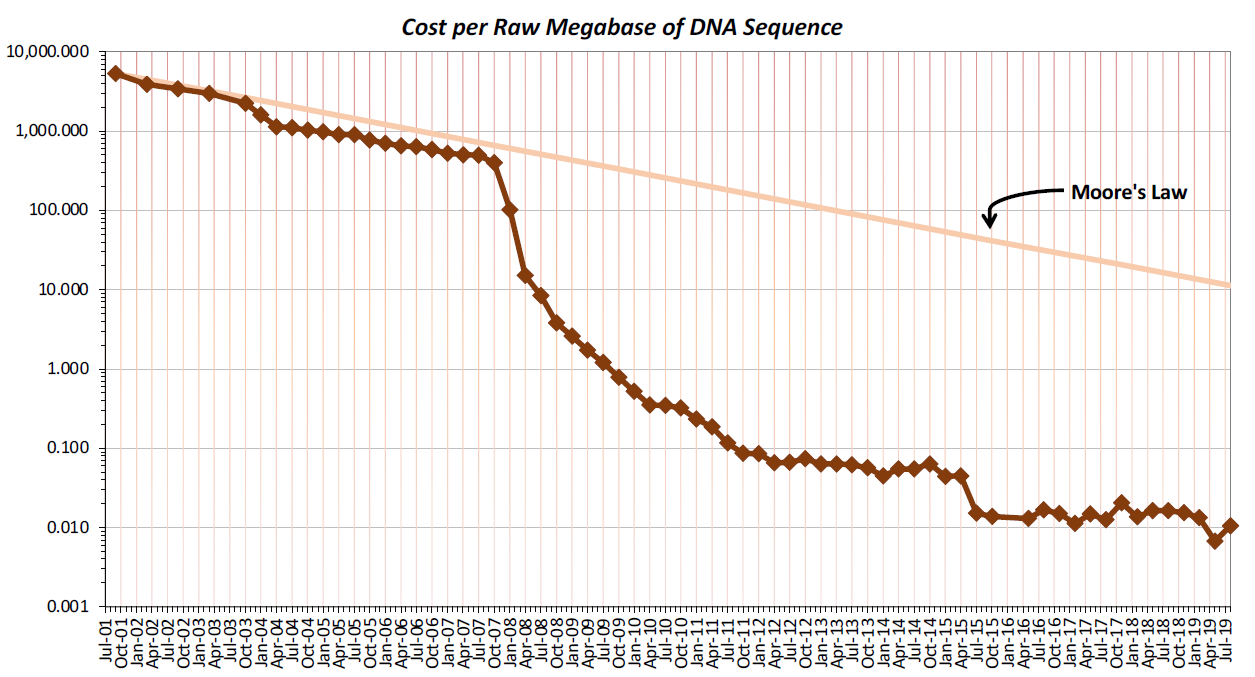
\includegraphics[width=0.6\textwidth]{sequencingCost}
\label{Moore's law graph}
\end{figure}

The methods of sequencing actually can be grouped in three \textbf{groups}, that are:

\begin{itemize}
	\item \textbf{Chemical degradation} of DNA: it includes the method of Maxam-Gilbert
	\item \textbf{Sequencing by synthesis (“SBS”)} which is the most common approach and the first to be developed. It uses DNA polymerases in primer extension reactions Illumina, Pacific Bioscences, Ion Torren and 454
	\item \textbf{Ligation-based}: sequencing using short probes that hybridize to the template, the technologies perteining to this class are SOLiD, Complete Genomics
	\item \textbf{Other:} Nanopores
\end{itemize}

\subsection{The Chain Terminators}

\begin{figure}[H]
    \centering
    \begin{subfigure}[b]{0.49\textwidth}
        \centering
        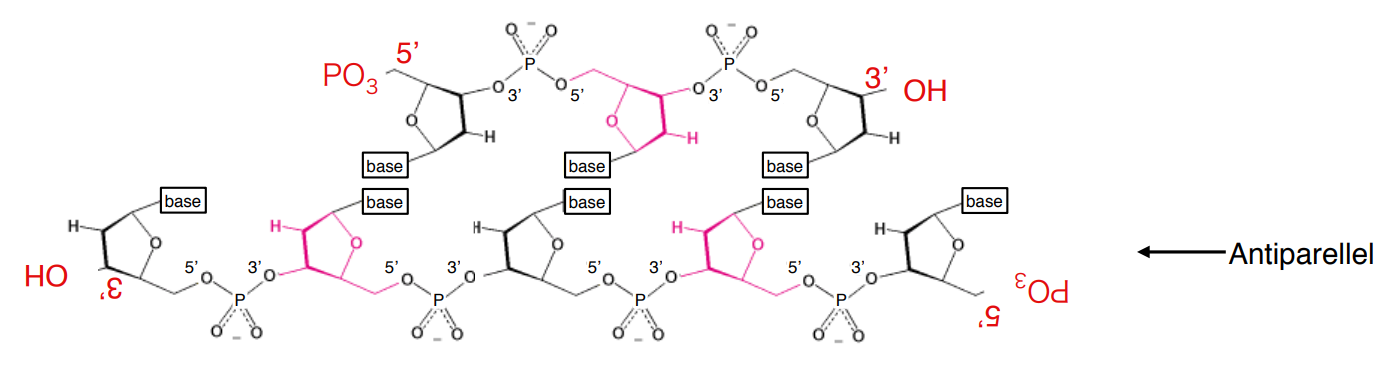
\includegraphics[width=\textwidth]{DNA-molecule}
        \caption{Normal DNA molecule, with oxydrilic group ligated to $3'$-ends}
        \label{normalDNAaddition}
    \end{subfigure}
    \hfill
    \begin{subfigure}[b]{0.49\textwidth}
        \centering
        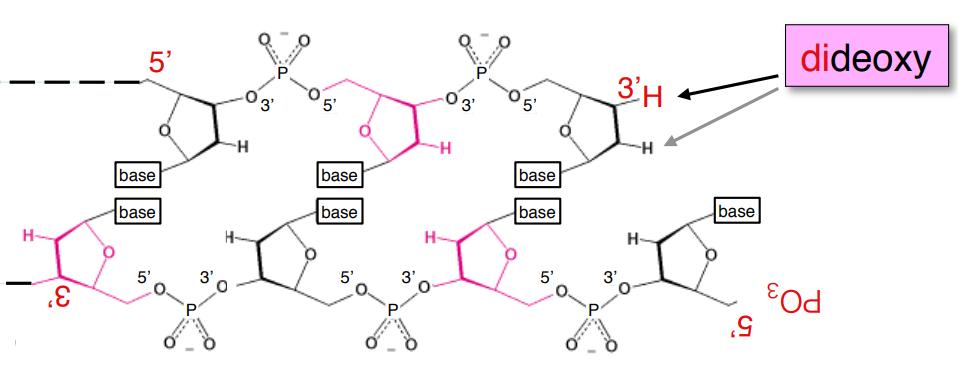
\includegraphics[width=\textwidth]{chain-term}
        \caption{Figure representing the difference between a normal DNA chain and one with chain terminators}
        \label{ChainTerm}
    \end{subfigure}
    \caption{Normal DNA synthesys \textit{vs} Chain terminators}
\end{figure}


Normally, the addition of new nucleotides to a generated molecule of DNA happens with the $3'$-end of the nucleotide chain (figure \ref{normalDNAaddition}). Chain terminators are dideoxy nucleotides, ddNTPs, that cannot be further extended. These nucleotides aren't able to add a new nucleotide on the $3'$-end, as they have not the needed oxydrilic group (figure \ref{ChainTerm}).

\subsection{Sanger method: the first one}

\begin{figure}[h]
\caption{The \textit{Sanger}'s method process}
\centering
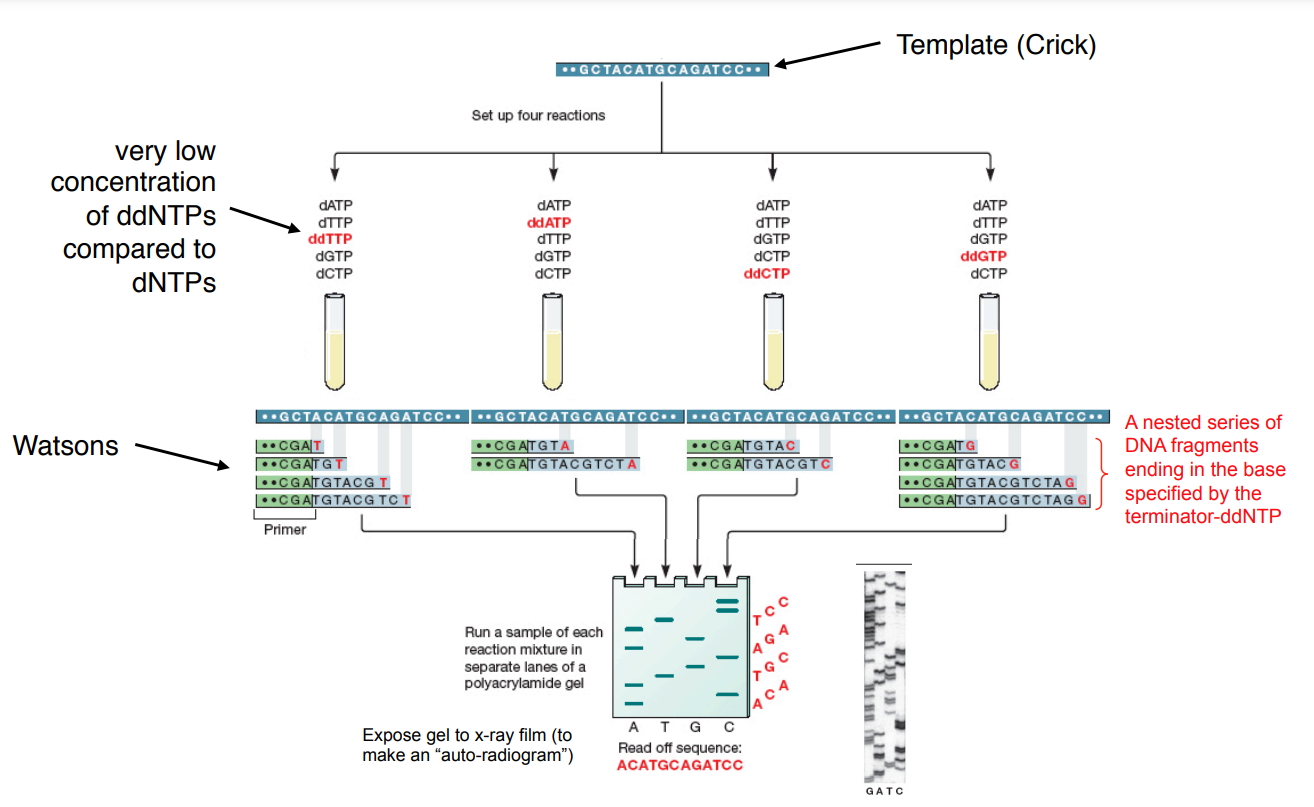
\includegraphics[width=\textwidth]{Sanger}
\label{Sanger}
\end{figure}

The first method ever used to sequence DNA was designed by Frederick Sanger. The Sanger manual sequencing system consists in an \textit{in vitro} process, which is described in figure \ref{Sanger}, also named as \textit{"primer extension"} method. It is performed over a single-filament DNA sample, and it uses the chain terminators nucleotides, a type for each nucleobase: ddATP, ddGTP, ddTTP, ddCTP.

The reaction is done inside four different reactions tubes, each containing the sample DNA to be reproduced, a DNA polymerase, the normal nucleotides and one of the four possible chain terminator. The chain terminators are marked with sulfur-35, a radioactive atom. In each tube, the corresponding dideoxy-nucleotide was used with a concentration 10 times lower than the other "normal" nucleotides.

From the polymerization reactions, several molecules of DNA were produced, with different length: each replicative cycle is in fact terminated after the addition of a chain terminator nucleotide.

To reconstruct the initial DNA sequence, a long PAGE gel was prepeared, with high concentration of urea ($6 - 7 M$) to avoid the coiling of the DNA single-filaments. To run the gel, high voltages were required and it had to be higly resolutive, as DNA's fragments are different only for a nucleotide. It was needed to do an auto-radiography of the gel in order to see the bands, in order to evidentiate the fosphorescent signals.

To read the sequence you have to start from the shortest fragments, at the end of the gel, and carefully go up along the gel, looking for the first presence of a band in one of the four runs. \\

\textbf{Past procedures: }In the past, the Klenow's fragment (part of the $1^{st}$ DNA polymerase) was used to perform the Sanger method, and the DNA to be sequenced was inserted inside the genome of an M13 phage.


\subsubsection{Automatic sequencing}
It does not use the radioactive signals, instead it uses fluorescent proteins. Several versions were developed after modifications of the Sanger method, in this order:

\begin{enumerate}
	\item fluorescent primers marked with a single fluorochrome.
	\item four aliquotes of the same primer were used marked with four different fluorochromes, able to emit different fluorescences.
	\item four different fluorochromes were used to mark the single ddNTPs
\end{enumerate}

Thanks to the use of 4 different fluorochromes, it was possible to use a single electrophoretic lane to carry the sequencing reaction. For this type of sequencing also, a cyclic replicative reaction was performed, with this procedure, made possible by using a thermal cycler:

\begin{enumerate}
	\item \textbf{Denaturation at $95$°C} of the DNA to be sequences
	\item \textbf{Annealing at $50-70$°C} of the primer specific to one of the two filaments
	\item \textbf{Extension at $72$°C} by using a \textit{Taq}-polymerase. The use of the Taq-polymerase makes it possible to avoid the formation of coiled structures in the DNA molecule to be sequenced.
\end{enumerate}

Traditionally, also in this type of sequencing it is used a long PAGE gel, as the Sanger's one, but with a great difference: all the ddNTPs are inserted in the same electrophoretic run, and after it, it is not needed an auto-radiography. Fluorescence, instead, can be triggered simply by irradiating the DNA molecules synthesyzed, which produce different fluorescences with different wavelengths.

\begin{figure}[h]
\caption{}
\centering
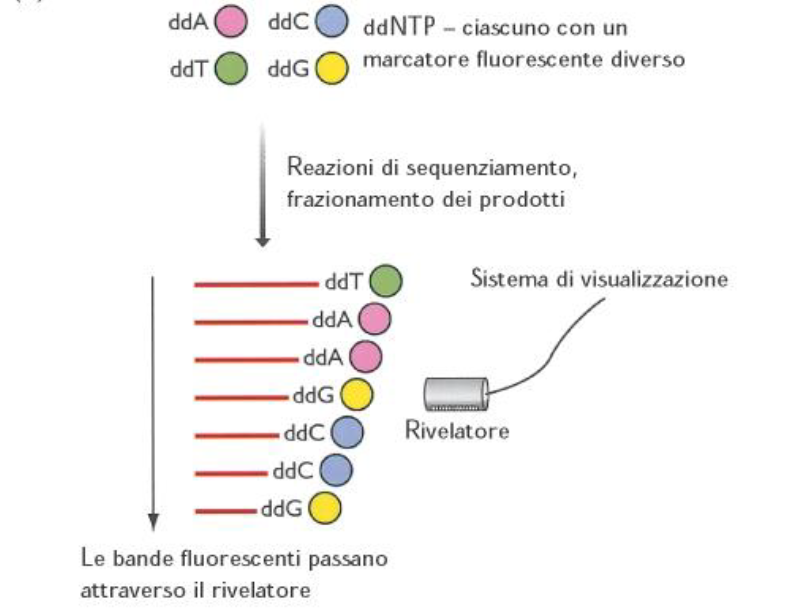
\includegraphics[width=0.8\textwidth]{automaticSang}
\label{}
\end{figure}


More usefully, this sequencing method is performed by using a capillar, filled with a synthetic polymer, with the same function of polyacrillamide.

At the end of the analysis, it is produced an electropherogram, with a color depicting the probability of each nytrogen base in each position. The production of the electropherogram is made better thanks to algorithms to boost signal/noise ratio, to correct the dye-effects, and other effects that generate systemic errors. %TODO dye-effects

\begin{figure}[h]
\caption{}
\centering
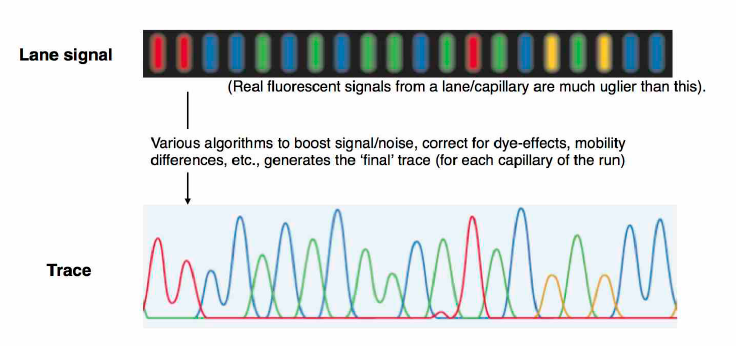
\includegraphics[width=0.8\textwidth]{elettroferogramma}
\label{}
\end{figure}

\begin{figure}[h]
\caption{The implementation of capillary sequencing machines gave the possiblity to make more runs than with the others. A $\tilde 1000$ fold productivity increase was allowed}
\centering
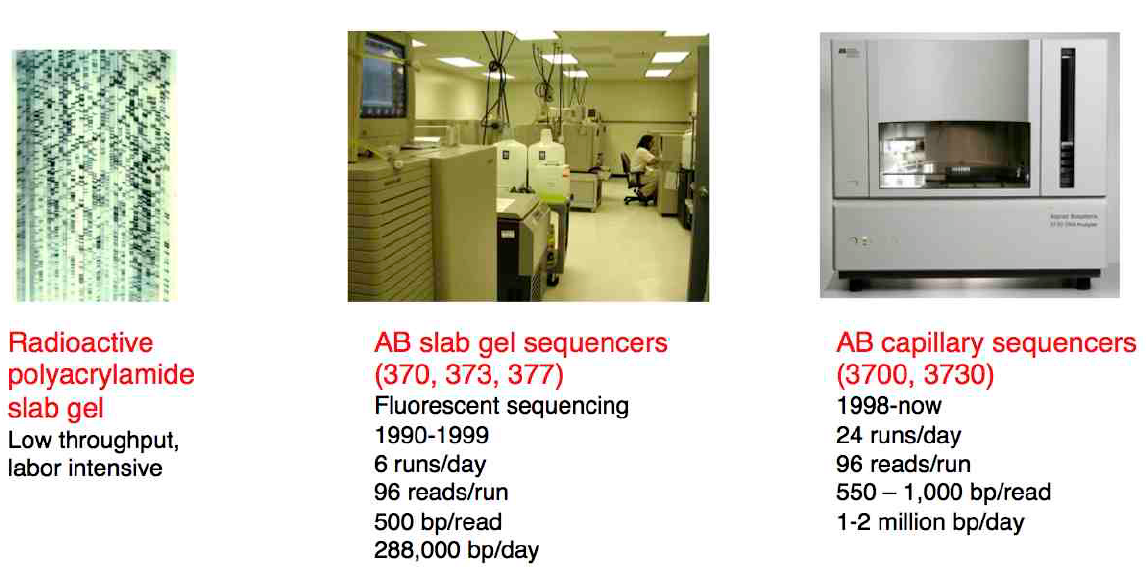
\includegraphics[width=0.8\textwidth]{progressSangerMachines}
\label{}
\end{figure}

Regarding the Sanger machines in use, the upgrades viewable in figure \ref{progressSangerMachines}. Based on the same technology, new machines were developed and it was obtained a $\tilde 1000$ fold improvement.
\\
When talking about the \textbf{human projec}t, it is important to specify that most of the job was done by using the Sanger automatic sequencing method.


\section{Development of Sequencing Machines}
The way you can get to the point could be different based on technology and the wanted output, comprised quality.

SOLID gave only $35$-$75$ sequenced bases, and it is not used anymore; Sanger sequencing, the capillary, can give up to 1000 read length, with a low output; on MINION it was possible to sequence an entire genome of \textit{E. coli}
A pletora of sequence machines are available today. None of the machines are able to sequence DNA from a sample of blood, some things have to be done. Nowadays \underline{machines producing bigger outputs of short reads are prefeared}.

\begin{figure}[H]
\caption{It can be noticed how recent developments had the scope of increasing the output data}
\centering
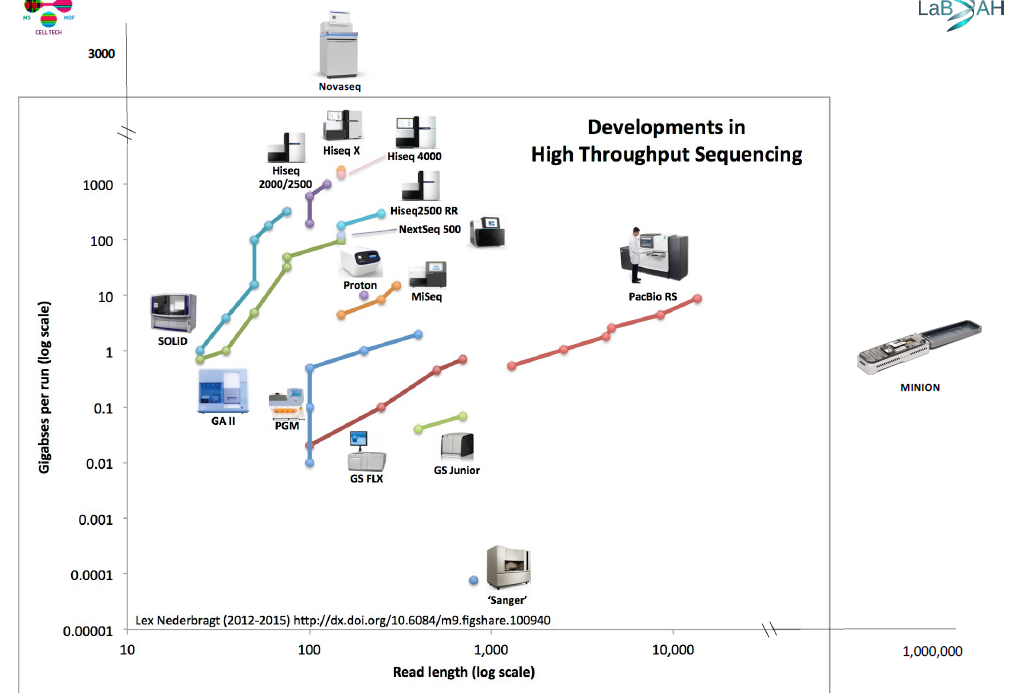
\includegraphics[width=1\textwidth]{sequencingMachines}
\label{}
\end{figure}

At the top of the market nowadays there are ILLUMINA machines, that use sequencing by synthesis method, NovaSeq is the biggest one. They need to amplify the signal through clusters formation.

\begin{figure}[H]
\caption{}
\centering
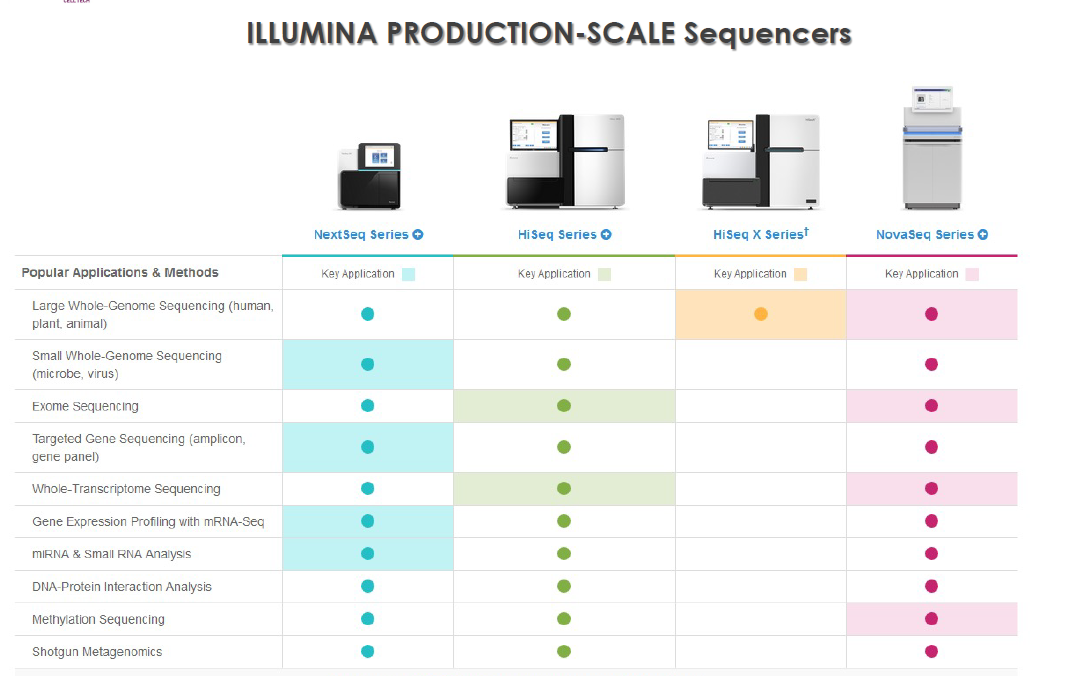
\includegraphics[width=0.8\textwidth]{sequencingMachinesIllumina}
\label{}
\end{figure}

\section{Next Generation Sequencing NGS}

The NGS protocol requires $3$ steps, that are:

\begin{enumerate}
	\item \textbf{Sample preparation}: series of fragments added
	\item \textbf{Clonal amplification}: which is is needed to replicate fragments attached to the solid surfaces, since machines are not sensible to single molecules
	\item \textbf{Sequencing}: ILLUMINA sequencing is one of the techniques used to obtain sequence data nowadays
\end{enumerate}

Tools pertaining to the $3^{rd}$ generation are those that permit to read a molecule without replicating it.

\subsection{Fragments/Library preparation}
Most of the sequences sequenced are fragmented in short read sequences, since most of the machines today used aren't able to sequence reads longer than some hundreds of nucleotides.

% Fragmantation is so required to generate shorter filaments from the sequences. In the case of mRNA (cDNA libraries) the fragmentation process is not needed, as the lengths are already short enough.

The fragments obtained have to be prepeared for the sequencing process, through a process called \textbf{tagmentation}. The obtained fragments are shown in the figure. Those fragments are provided with one or two indexes, called also barcodes, two sequencing primer binding sites and regions complementary to the oligonucleotides present in the chamber (see in Clonal amplification chapter). The fragments' length has to be checked, depending on the scope of the process. Indexes are needed to run sequencing process on multiple samples, they are needed to distinguish those; when they are two, they permit to distinguisch also the 2 types of sequencing that are performed, forward and reverse.

P5 and P7 are the oligos needed to attach fragments to ILLUMINA sequencing machines.

\begin{figure}[h]
\caption{Figure representing the a good prepeared fragment, it has two indexes, two sequencing primer binding sites and regions complementary to the oligonucleotides present in the chamber}
\centering
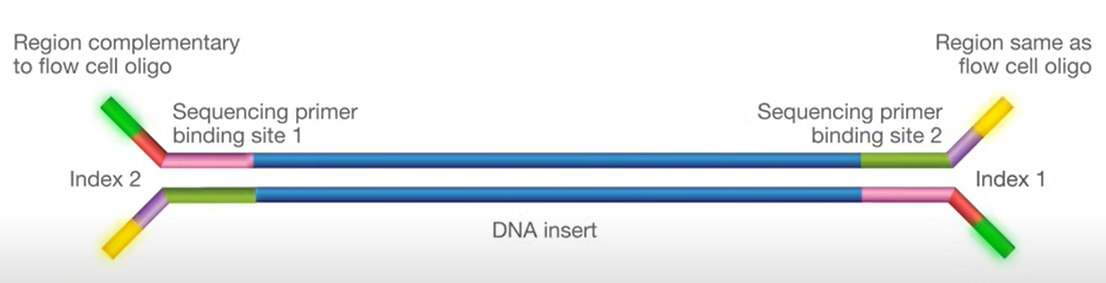
\includegraphics[width=0.8\textwidth]{tagmentedFragments}
\label{}
\end{figure}

%what is a good fragment? %TODO

\subsection{Clonal amplification and ILLUMINA sequencing procedure}

\begin{figure}[h]
\caption{}
\centering
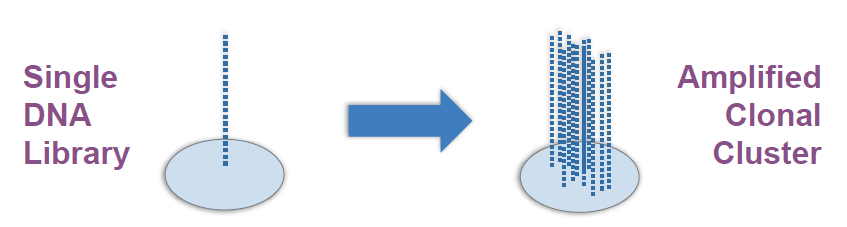
\includegraphics[width=0.6\textwidth]{clusterAmplification}
\label{clusters}
\end{figure}

Clonal amplification are necessary to amplify the signal from each single fragment.
ILLUMINA machines make use of clusters to sequence DNA. Clusters are a group of DNA
strands positioned closely together and generated from a single DNA filament. Generally, Each cluster represents thousands of copies of the same DNA strand in a 1–2 micron spot (figure \ref{clusters}).

\begin{figure}[h]
\caption{}
\centering
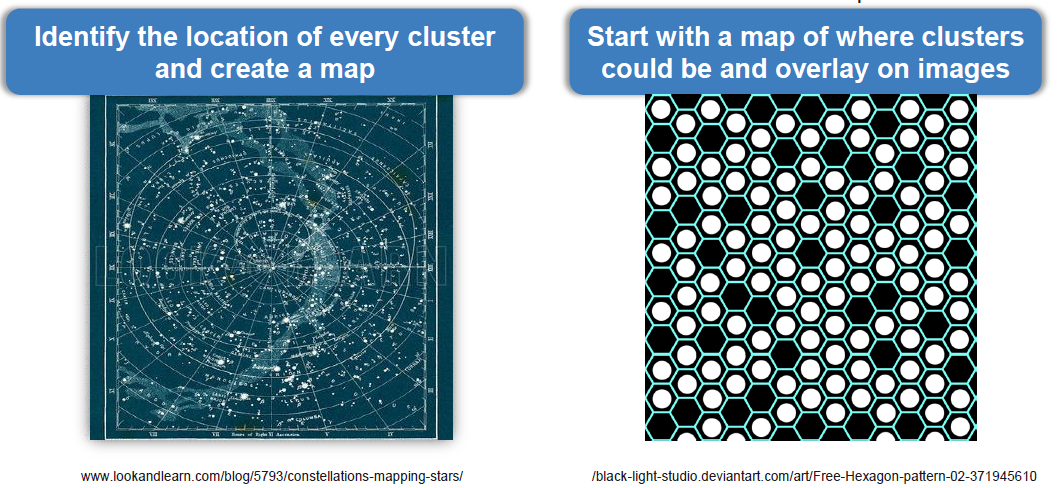
\includegraphics[width=0.8\textwidth]{rigidGeneration}
\label{rigid}
\end{figure}

On patterned flow cells, the clusters' formation location could be known or not, in the first case it is said that there is a "Rigid registration" (figure \ref{rigid}).\\


ILLUMINA sequencers normally use slides of glass, named flow cells, and the fragments to be sequenced are able to flow over the channels. The temperature inside the cells can be changed to produce ligations or separations. The surface of the cells is functionalized with a series of oligos complementary to library adapters.

Two kids of flow cells, the \textit{patterned} flow cell permits to create clusters in specific positions, inside nanowalls, contrarily to \textit{Random Flow Cell} which instead have randomly positioned clusters.
\begin{figure}[h]
\caption{}
\centering
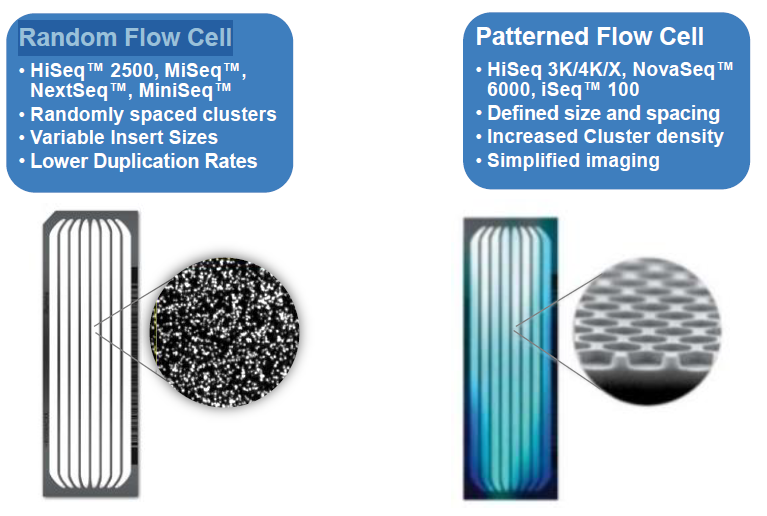
\includegraphics[width=0.6\textwidth]{randomPatternCells}
\label{}
\end{figure}
\\

Once the fragments are made flow over the chambers, they can bind only to p5 or p7 (ILLUMINA oligos), the two oligos functionalizing the plate. Once the fragments are attached to the surface, using temperature and solvents flows you can control the sequencing process. To see the entire procedure:
(procedure on Youtube: \href{https://www.youtube.com/watch?v=womKfikWlxM}{video about ILLUMINA sequencing}). In the video, it is shown the two index sequencing process.
\\
\\


\begin{figure}[H]
    \centering

    \begin{subfigure}[b]{0.39\textwidth}
        \centering
        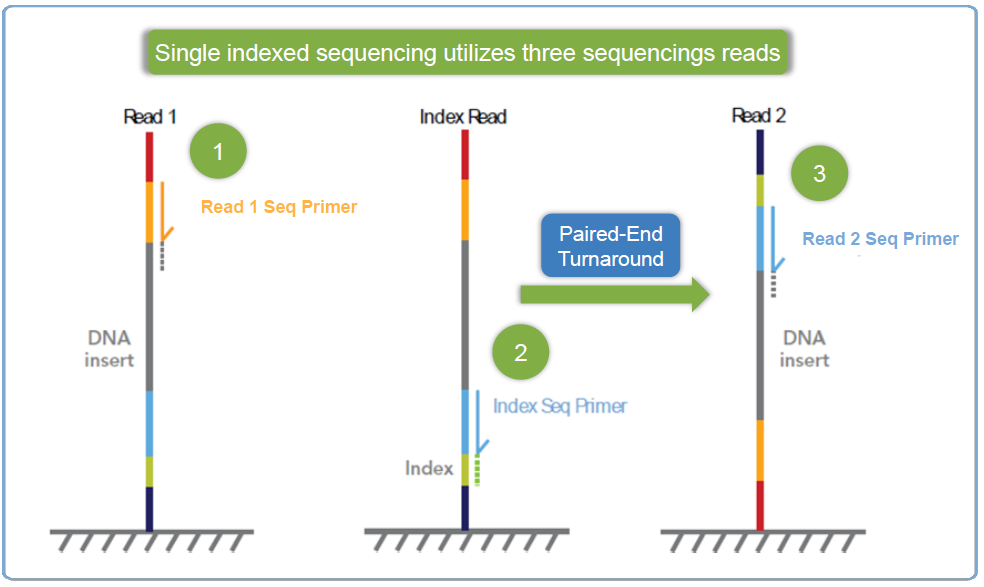
\includegraphics[width=\textwidth]{singleIndex}
        \caption{single index}
    \end{subfigure}
    \hfill
    \begin{subfigure}[b]{0.60\textwidth}
        \centering
        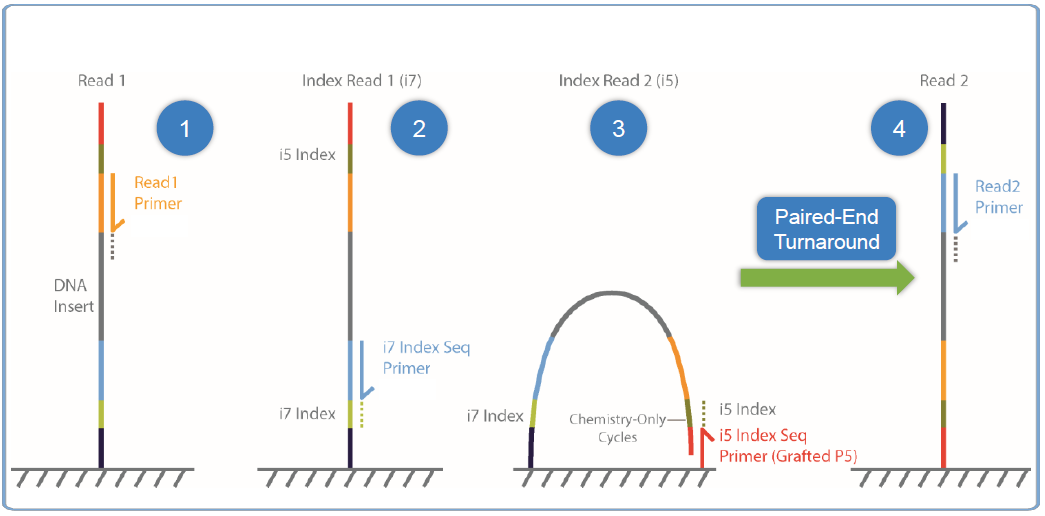
\includegraphics[width=\textwidth]{doubleIndex}
        \caption{double index}
    \end{subfigure}
    \caption{Single/double index for ILLUMINA sequencing}
    \label{singDoubInd}
\end{figure}

With 1 and 2 indexes the sequencing process actually differs, as shown in figure \ref{singDoubInd}


\begin{figure}[H]
\caption{}
\centering
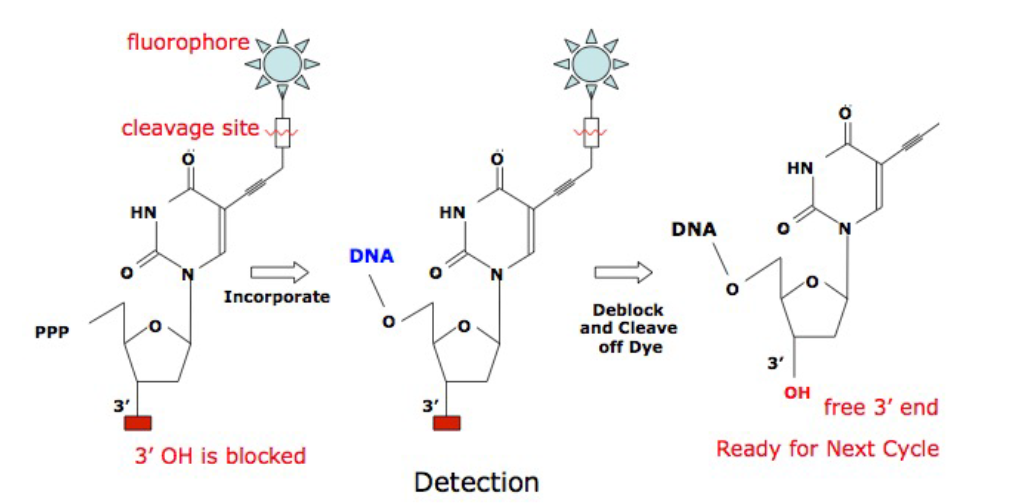
\includegraphics[width=0.7\textwidth]{ILLUMINArev}
\label{ILLUMINArev}
\end{figure}

To perform the sequencing process, ILLUMINA machines utilize \textit{reversible terminators} (figure \ref{ILLUMINArev}). They permit a real time analysis of the sequencing by synthesys reaction, and because of this they are different from the Sanger method. Fluorophores are reversible, they can be cleaved to eliminate the light signal.

\begin{figure}[h]
\caption{}
\centering
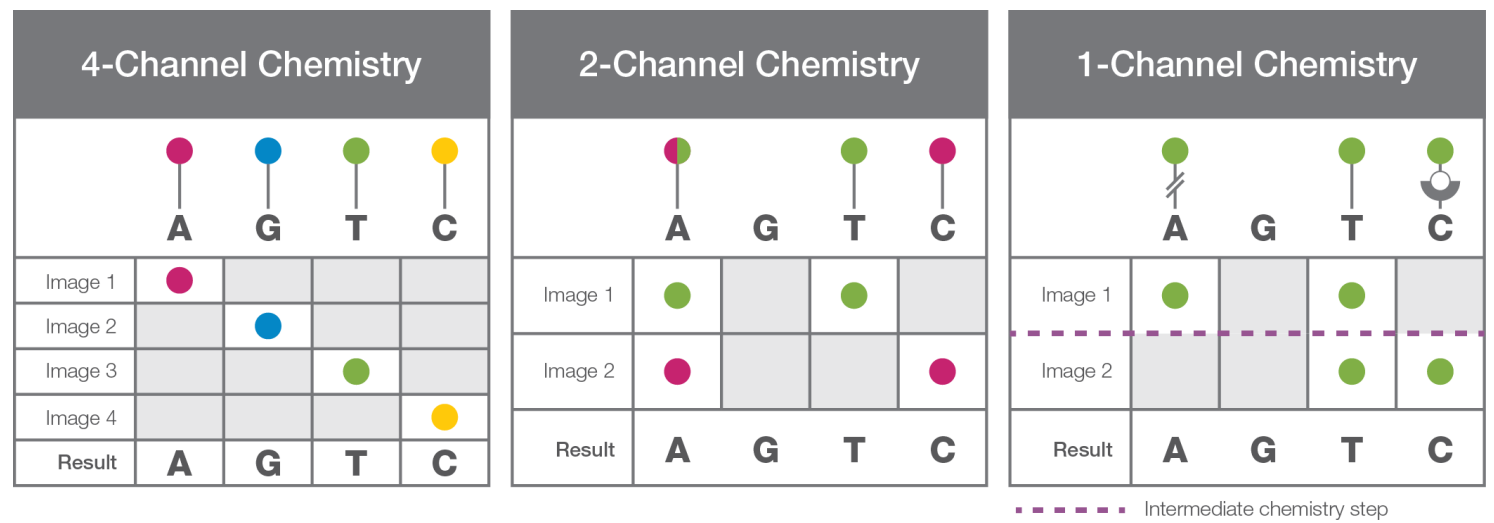
\includegraphics[width=0.8\textwidth]{ChannelILLUMINA}
\label{ChannelILLUMINA}
\end{figure}

To perform their activity, ILLUMINA sequencers could be of 3 different types: 4-Channel, 2-Channel or 1-Channel, depending on the number of fluorescent molecules used. In the case of the 4-Channel technology, 4 images are taken in each cycle, and each  cluster appears in only one of four images \ref{ChannelILLUMINA}. 2-Channel technique is used by some sequencing machines, like NextSeq 550, MiniSeq, NovaSeq 6000\\

4-Colors base calling
is needed to to make
the true signal the purest, and after, The base with the highest intensity becomes the called base for that cluster. In the case no base is clearly related to a position, \textit{N} is the result.


The reading process could be done in two ways: through single reads, on a single extreme of the fragments, of paired-end, on both the extremes. The second one in particular gives structural and 2 sequence  informations.


\subsection{Pacific Bioscience (PacBio)}
the long DNA filement to be sequenced is attached to a polymerase, over the surface of a SMRT (Single Molecule Real Time) cell. This cell is really small, and at each nucleation process a light signal is emitted. The produced light is not able to get out of the walls, and its duration is extremely restricted. Sequencing, also in this case, is made by sequencing, and the main advantage consists in the possiblity of sequencing really big DNA molecules.\\
In the video \href{https://www.youtube.com/watch?v=_lD8JyAbwEo}{PacBio procedure} it is briefly shown how the process works and what are the strategies used to reduce errors.

\begin{figure}[h]
\caption{}
\centering
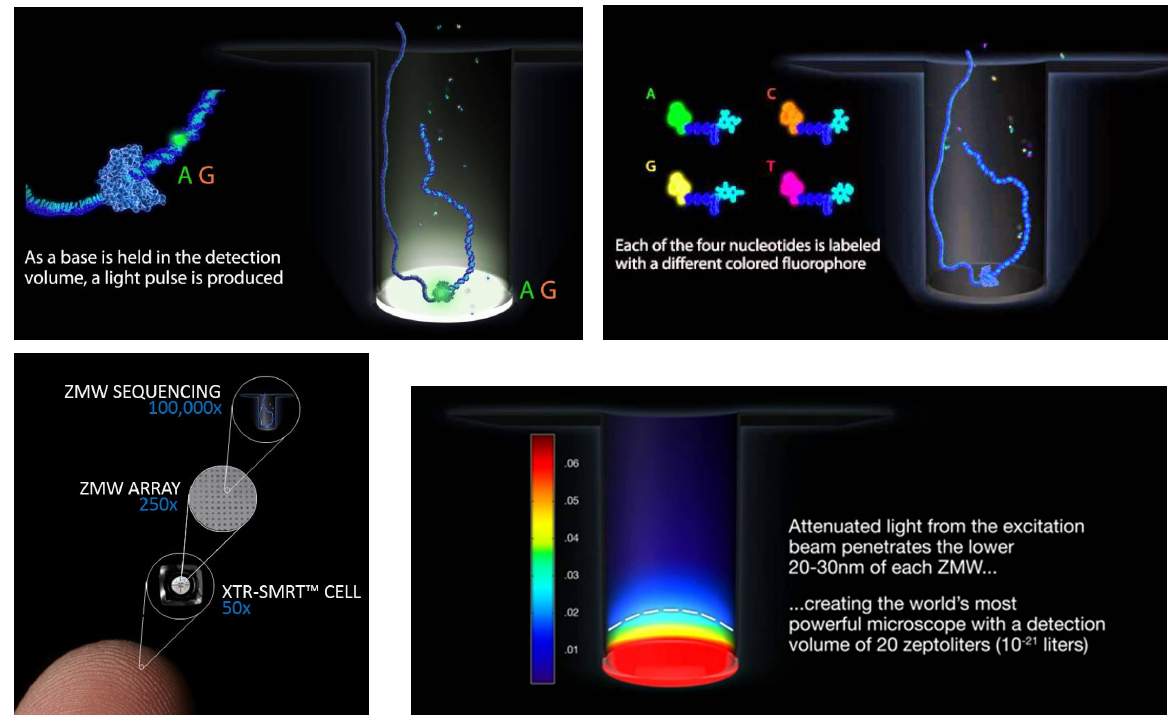
\includegraphics[width=1\textwidth]{PacBIO}
\label{}
\end{figure}


\subsection{Nanopore sequencing}
Intramembrane proteins are used, sequence detected through the passage of DNA nucleotides, which produce different voltage changes. During the first periods, this type of instruments gave great amount of errors, nowadays the technique is improving.
\href{https://www.youtube.com/watch?v=E9-Rm5AoZGw}{Nanopore Sequencing}
